\documentclass[a4paper,10pt,oneside]{article}
\usepackage[utf8]{inputenc}
\usepackage[english]{babel}
\usepackage{hyperref}
\usepackage{tabularx}
\usepackage{booktabs}
\usepackage{longtable}
\usepackage{graphicx}
\usepackage[font=small,labelfont=bf,tableposition=top]{caption}
\usepackage{subcaption}
\graphicspath{ {./images/} }

\hypersetup {
        colorlinks=true,
        linkcolor=blue,
        anchorcolor=black,
        filecolor=magenta,
        urlcolor=cyan,
        citecolor=blue
}

%opening
\title{Human Activity Recognition With Smartphones}
\author{Jeremy Sapienza, Simone Fiorellino, Stefano D'Arrigo}

\begin{document}

\maketitle



%sds

\section{Introduction}
Nowadays everyone has a smartphone in his pocket and carries it everywhere he goes during the day journey. Smartphones collect each time a huge amount of data through their embedded sensors. High tech industries are involved into the development of accurate wearable devices to improve every day life, monitoring the activities of their customers, from walking in a park to laying on the bed.\\
%Hence, it would be valuable to leverage the information coming from mobile devices to recognize human activities. Useless to say, high classification performance is strongly required.
Hence, we reckoned this topic valuable and in our project we focused on the classification task of human activities, making use of accelerometer and gyroscope records. Our attention was particularly concentrated on the training of two classifiers, GDA and SVM,  and on the research of a convenient data representation.
In this report we summarize the methods we applied and the choices we made. Finally, in the last section we present our findings and give some further analyses.


\section{Related work}
For this work we were inspired by the paper \cite{brown2013activity}.
Their research focused on developing a classifier that operates on accelerometer and gyroscope data from mobile phones.
As explained in \cite{anuita2013human}, they recorded the stream of data of 30 subjects during different types of activities: walking, walking up stairs, walking down stairs, sitting, standing and laying (Figure \ref{fig:classes}).

\begin{figure}
 \center
 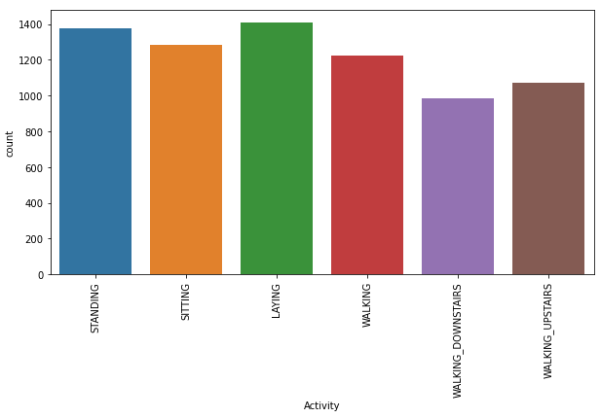
\includegraphics[width=0.6\textwidth]{class_distro}
 \caption{Number of samples of each class. As we can see, the dataset is almost balanced.}
 \label{fig:classes}
\end{figure}

\noindent The dataset have two types of data:
\begin{itemize}
 \item “Raw data”: raw gyroscope and accelerometer readings.
 \item “Preprocessed data”: vectors of  561 features that represent 2.56s of time. These features are the result of different functions, some examples are: triaxial average, maximum and minimum acceleration, angular velocity (over the given interval) or Fourier transform.
\end{itemize}

\noindent They used for this part of work the preprocessed data.

\noindent To approach this problem they used three different models:
\begin{itemize}
 \item Naives Bayes
 \item GDA
 \item GDA + Hidden Markov Model
\end{itemize}

\begin{table}[ht]
\centering
\begin{tabular}{p{0.35\textwidth} p{0.35\textwidth}} 
\toprule
\textbf{Algorithm} & \textbf{Accuracy}\\[5pt]
\midrule
Naive Bayes & 80\% \\[5pt]
GDA & 96\% \\[5pt]
GDA + HMM & 98\%\\[5pt]
\bottomrule\\[5pt]
\end{tabular} 
\caption{Results of the analysis of paper \cite{brown2013activity}.}
\label{tab:paper}
\end{table}

\noindent Reffering to Table \ref{tab:paper}, the GDA accuracy is much higher than the Naive Bayes model because this last model makes the assumption that the features are independent of each other. But, in this context, having the features more correlated together, the accuracy with the Naive Bayes model is pretty low.
Another important aspect of this paper is the dimensionality reduction. They used the PCA in order to decrease the computational complexity of the model and improve the accuracy.


\section{Methods}

\subsection{Data preprocessing}
We retained 60\% of the data for the models' training; the remaining part was equally splitted into evaluation and test sets.
 
\subsection{Models}
As a first step, we implemented the Gaussian Discriminant Analysis classifier and trained it on the data; the choice of this model was mainly conditioned by \cite{brown2013activity}. For the implementation, we faced out with the problem of multiclass classification, as in \cite{guillame2020, bamtak}. With the purpose of improving the performance, we took into account a step of feature selection and dimensionality reduction: indeed, the high number of derived features forced us to focus on the relationship between the features of the original dataset, the variance of them and the predicted classes. So, we considered two different strategies:
\begin{itemize}
 \item feature selection with the Analysis of Variance model (ANOVA);
 \item dimensionality reduction with the Singular Value Decomposition method (SVD) (Figure \ref{fig:var}).
\end{itemize}
The second step was training the Support Vector Machine classifier on the data, following the same approach just described. After reviewing \cite{james2013introduction, aggarwal2015data, ma_ng_re_2009, bishop2006pattern} and having tried to implement it as in \cite{platt1998sequential, kowalczyk2017support}, we decided to use the implementation given by the library “Scikit Learn” \cite{scikit-learn, sklearn_api}. In this case, it was essential finding a good configuration of feature space and model hyperparameters. Since this research would have taken too much to be conducted on each possible combination of hyperparameters, we chose a set of them which we reckoned reasonable.\\ The results of the training and fine tuning step will be presented and commented on in the next section.


\begin{figure}
 \center
 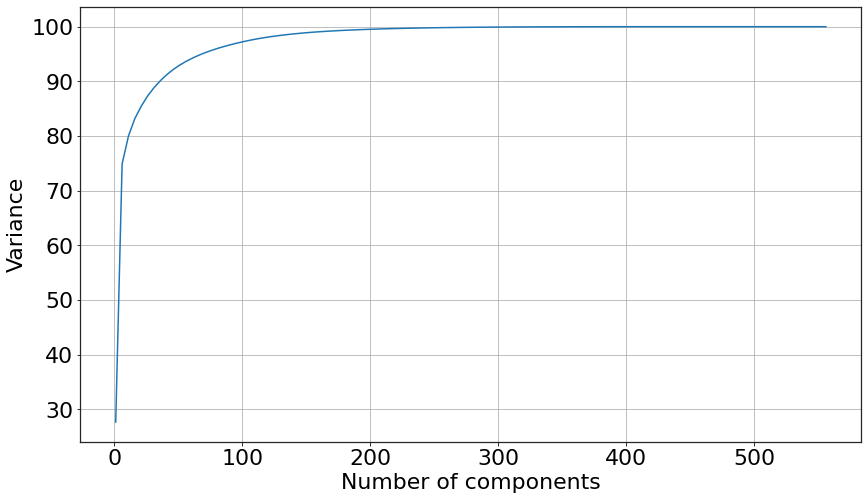
\includegraphics[width=0.6\textwidth]{components_variance}
 \caption{Feature variance with respect to the number of components after the application of the SVD method. The plot confirms that many features are not very discriminant: almost 100\% of the variance is retained with just 200 components.}
 \label{fig:var}
\end{figure}

\section{Experimental results}
\subsection{GDA results}
Initially the model led to an accuracy of 94\% on the whole feature space. Instead, by applying the dimensionality reduction we improved the score, obtaining an accuracy of 97\%.
In this model, \textit{sitting} and \textit{standing} are the classes with lowest performance, as we can see in the confusion matrix (Figure \ref{subfig:1}). 

\subsection{SVM results}
As we can see in the confusion matrix (Figure \ref{subfig:2}), SVM got a better performance than the GDA model, 99\% of accuracy.
The results we obtained are compliant to our expectations, indeed:
\begin{itemize}
 \item The GDA carried out the same performance of the reference paper \cite{brown2013activity}.
 \item Support Vector Machine led to the best results exceeding those of references.
 \item We improved the performance of our model through the dimensionality reduction and the choice of good hyperparameters.
\end{itemize}


\begin{figure}[ht]
 \center
 \begin{subfigure}{0.45\textwidth}
  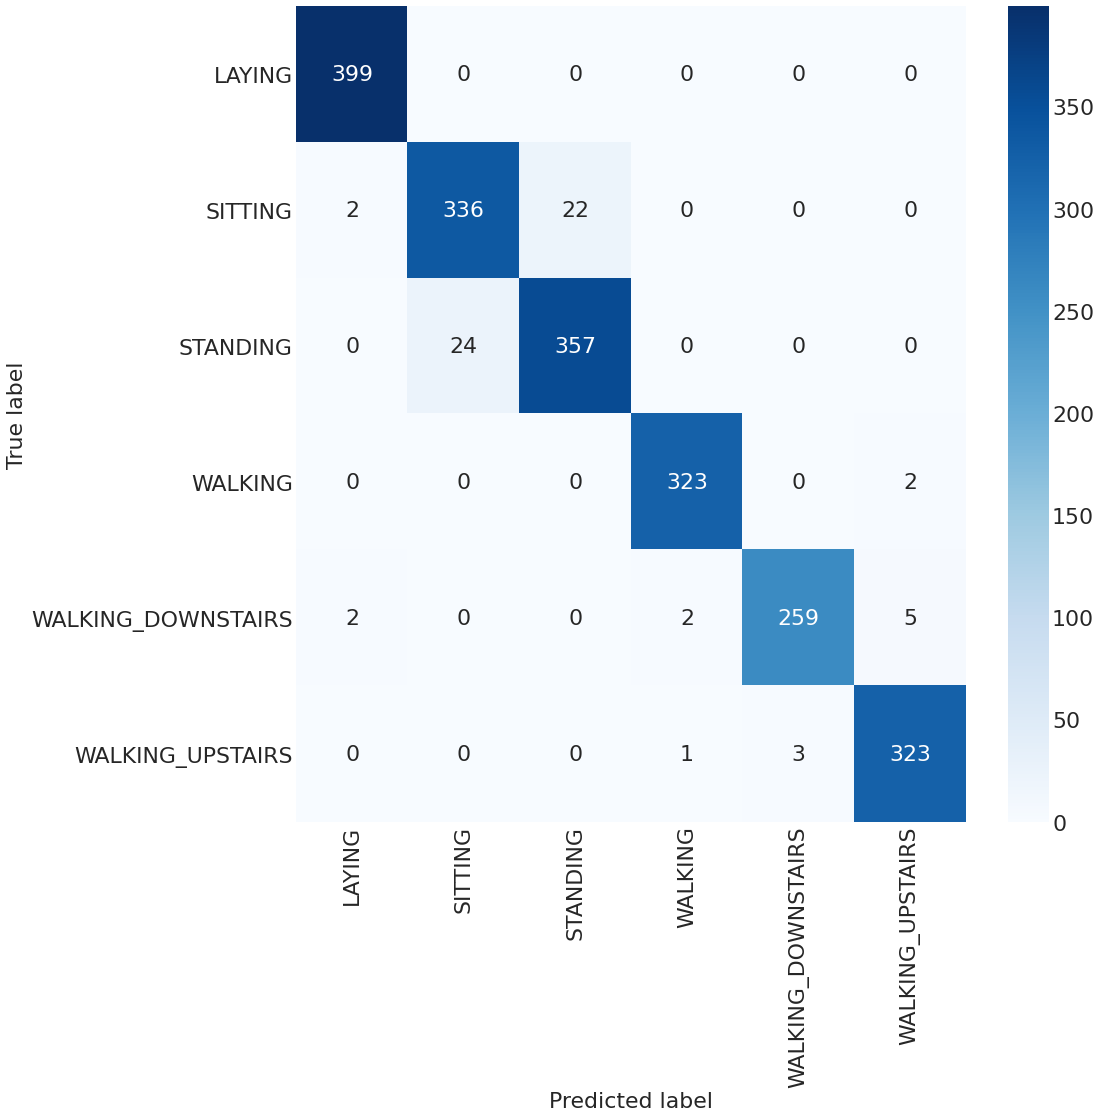
\includegraphics[width=\linewidth]{conf_mat_gda}
  \caption{}
  \label{subfig:1}
 \end{subfigure}
 \begin{subfigure}{0.45\textwidth}
  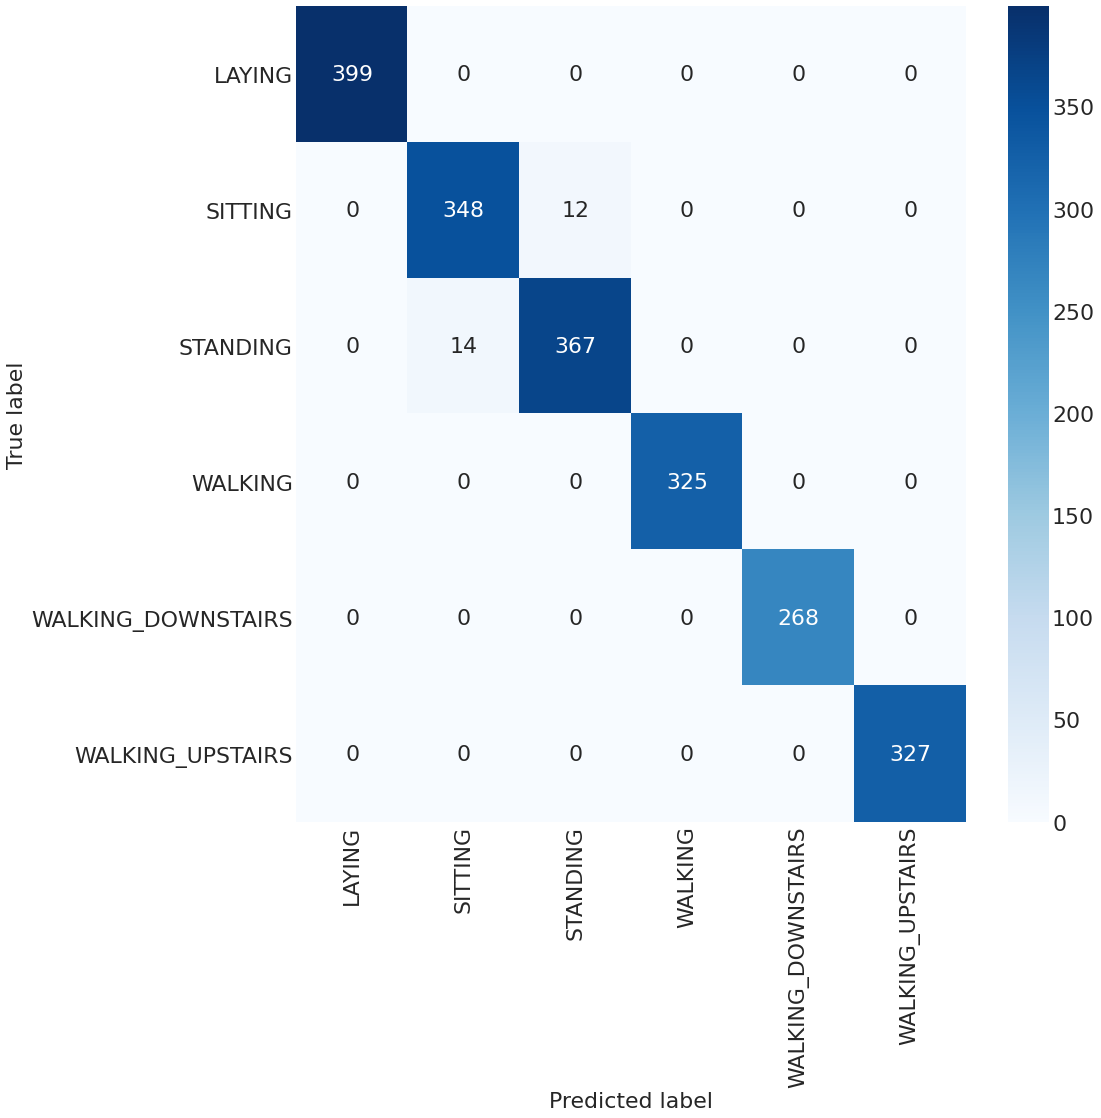
\includegraphics[width=\linewidth]{conf_mat_svm}
  \caption{}
  \label{subfig:2}
 \end{subfigure}
 \caption{Confusion matrices of GDA (fig.\ref{subfig:1}) and SVM (fig.\ref{subfig:2}).}
 \label{fig:conf_mat} 
\end{figure}

\section{Conclusion and future work}
The results we got were quite impressive, cause we managed to reach a very high preformance score. 
As a future work, it would be worth handling the raw data, in order to elaborate the data without preprocess them.

\vspace{0.3cm}

\bibliography{references}
\bibliographystyle{abbrv}

\end{document}
